\section{Introduction et Objectifs}


\section{Gestion de Projet : Diagramme de Gantt}
\begin{figure}[H]
	\centering
	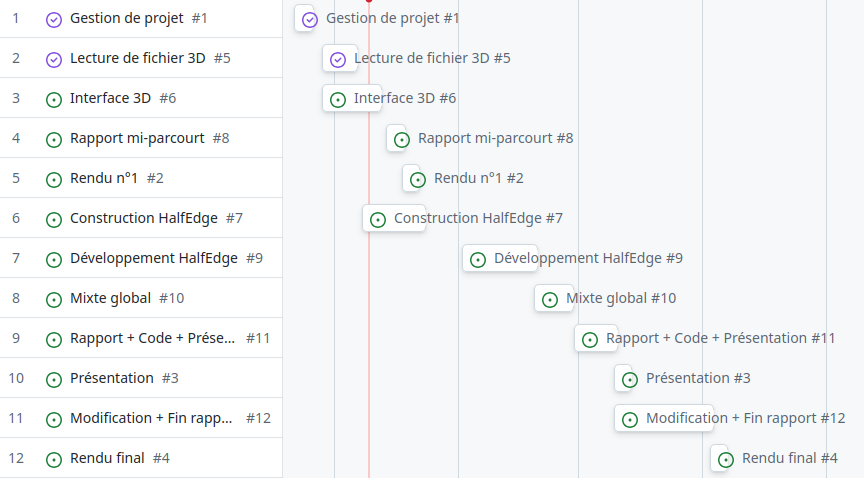
\includegraphics[width=0.7\linewidth]{Image/Gantt}
	\caption{Diagramme de Gant}
	\label{fig:gantt}
\end{figure}


\section{Architecture Logicielle et UML}
Avant de débuter la phase de programmation et d'écriture du code, il est essentiel de concevoir l'architecture du projet. C'est l'un des principes fondamentaux de la programmation orientée objet. Pour ce faire, l'outil le plus répandu et efficace est le diagramme de classes UML, qui permet de visualiser la structure des classes ainsi que leurs interactions. 
\begin{figure}[H]
	\centering
	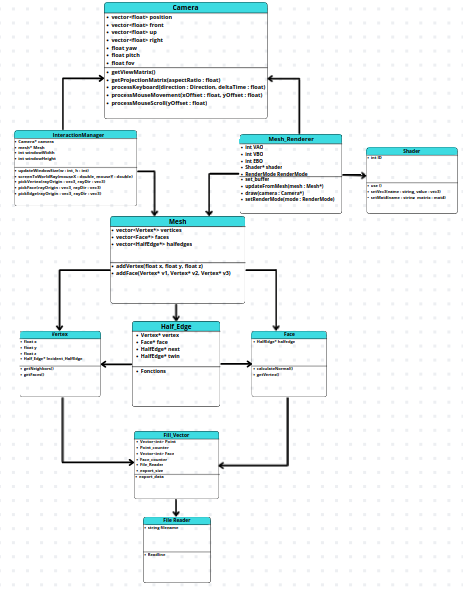
\includegraphics[width=0.7\linewidth]{Image/UML_Complet}
	\caption{Diagramme UML}
	\label{fig:umlcomplet}
\end{figure}
Ci-dessus, nous pouvons voir notre diagramme UML avant programmation. Il est évident que celui-ci est voué à être un peu modifié, car nous pourrons être confrontés à des problèmes futurs qui devront être résolus à l'aide de fonctions ou de classes auxquelles nous n'avions pas encore pensé.
\newline
\newline
Notre diagramme UML a été structuré en deux parties principales. La première concerne la structure Half-Edge, regroupant l'ensemble de la chaîne de traitement, du chargement des données du fichier .obj jusqu'à la construction des vecteurs de demi-arêtes. 
\newline
La seconde partie est dédiée à OpenGL et au rendu graphique. Cette dernière est la plus susceptible d'évoluer, car elle repose sur des concepts que nous maîtrisons moins pour le moment, notamment la gestion de la caméra et des shaders, indispensables sous OpenGL.  
\begin{figure}[H]
	\centering
	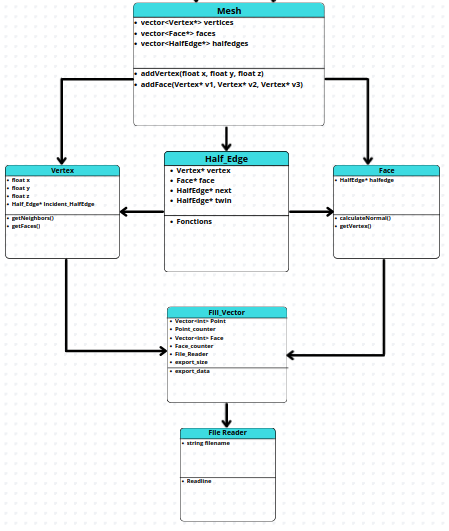
\includegraphics[width=0.7\linewidth]{Image/UML_halfedge}
	\caption{UML de la partie Half edge}
	\label{fig:umlhalfedge}
\end{figure}
\begin{figure}[H]
	\centering
	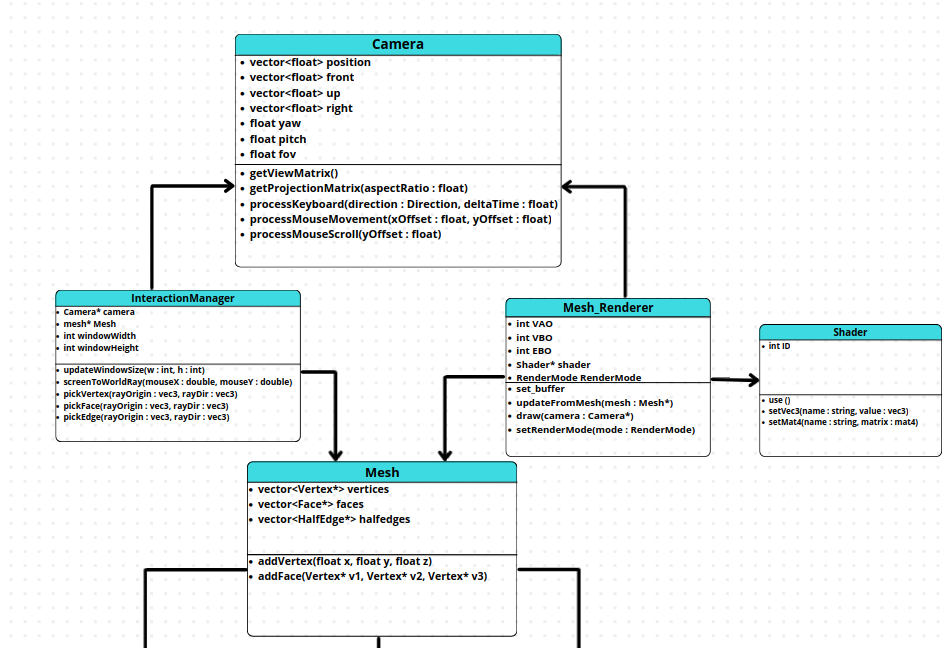
\includegraphics[width=0.7\linewidth]{Image/UML_OpenGl}
	\caption{UML de la partie OpenGL}
	\label{fig:umlopengl}
\end{figure}

\section{État d'avancement du projet}


\section{Analyse des Risques et Plans B}
